\section{Illustration}
%\section{Experimentations}

To illustrate our theoretical results, we evaluate the predictive performance and the ability of the models to capture homophily and preferential attachment on artificial and real networks. In the sequel, we first describe the measures used to evaluate the properties of interest and the predictive performance, then the datasets used in our experiments. Afterwards, we detail the evaluation protocol and we present the experimental results.

\subsection{Homophily Measures}

For the homophily property, defined in section \ref{sec:homophily}, we represent using boxplots, the distributions of the similarity natural $s_n(i,j)$ and latent $s_l(i,j)$ computed respectively on linked and non-linked pairs of nodes. Note that for all the models the values are aggregated on the datasets andd reported as final results.
% The links or non-links are obtained by running the models in a generative mode. For each models we aggregated  the similarity of each couple of nodes as well as link prediction (links or non-links). The distributions of similarities are then represented on a boxplot that shows how the they are spread according to links and non-links.


\subsection{Preferential attachment Measures}
\label{sec:experiments-burst}

The measures considered to evaluate the preferential attachment rely on a goodness of fit. Indeed, it has been reported that preferential attachment leads to networks characterized by a degree distribution with heavy tail drawn from a power law. A graphical method, most often used to verify that the observations are consistent with this law  consists in constructing the histogram representing the degree distribution and if the plot on doubly logarithmic axes approximately falls on a straight line, then one can assume that the distribution follows a power law. Thus, the comparison of the degree distribution in the log-log scale with a linear function gives us a qualitative measure for the preferential attachment. To obtain a second evaluation of the power law hypothesis for the degree distribution, we follow the statistical framework, introduced by \cite{clauset2009power}, for discerning and quantifying power-law behavior in empirical data. This framework combines maximum-likelihood fitting methods with goodness-of-fit tests based on the Kolmogorov-Smirnov statistic to compute $p$-value.

If  $p$-value is large (close to 1), then the difference between the data and the model can be attributed to statistical fluctuations alone; if it is small, the model is not a plausible fit for the data and we can not conclude that there is an evidence for the preferential attachment in the network. 


%In the context of latent models, while there is no ambiguity in computing the overall degree distribution, it is less obvious for the local case. We explain here the computation of the local degree distribution for each models according to section \ref{sec:burstiness} :
Concerning the local preferential attachment, 
the computation of the local degree distributions for each model is detailed below: 
\begin{itemize}
    \item For each network learned with IMMSB, the tensor $Z$ indicates the membership of the nodes for each  interaction. In order to draw the local degree distribution for a factor $k$, we reduce the adjacency matrix in order to retain only the links that occur for the factor $k$. The local degree distribution is thus computed on the reduced adjacency matrix  $Y^k =\{ y_{ij}^k=1 \ \textrm{if}\ y_{ij}=1 , z_{i\rightarrow j}=k, z_{i\leftarrow j}=k; 0 \ \textrm{otherwise} \}$.
        \item For ILFM, each node $i$ is associated with a feature vector $\mat{f}_{i}$. The local degree distribution for the factor $k$ is obtained by taking into account only the contribution of this feature $k$ on the adjacency matrix. Thus, the local degree degree distribution is computed on the reduced adjacency matrix defined by $Y^k =\{ y_{ij}^k=1 \ \textrm{if}\ y_{ij}=1 , f_{ik}=1, f_{jk}=1; 0 \ \textrm{otherwise}\}$.
\end{itemize}


\subsection{Prediction performance evaluation}
The prediction problem is equivalent to a binary prediction problem which consists to decide for each pair of nodes if there is an edge or not between them. 
Thus, the performance of the models can be evaluated with usual AUC-ROC measures and curves which allow to graphically compare the predictive performance of the models on each dataset.

\subsection{Training Datasets}

In our experiments, we consider two artificial networks and two real networks.  Main topological characteristics of these networks are summarized in Table \ref{table:networks_measures} and we describe those networks in the sequel.

\begin{table}[h] 
	\centering
	\caption{Characteristics of artificial and real networks.}
	%\resizebox{\textwidth}{!}{  
    \begin{tabular}{lrrr}
        \hline
        \textbf{Networks} &   nodes &   edges &   density \\
        \hline
        Network1 &    1000 &    3507 &     0.007 \\
        Network2 &    1000 &   31000 &     0.062 \\
        Blogs         &    1490 &   20512 &     0.009 \\
        Manufacturing &     167 &    5950 &     0.215 \\
    \hline
    \end{tabular}
	\label{table:networks_measures}
\end{table}

The non-oriented artificial networks (Network1 and Network2) have been generated with DANCer-Generator \cite{largeron2015}. This generator has been chosen because it allows to build an attributed graph having a community structure  and  the known properties of real-world networks such as preferential attachment and homophily.
Moreover, by modifying the parameters, these properties can be weakened. Finally, DANCer-Generator is available under the terms of the GNU Public License and the parameters can be shared for experiments reproducibility. Furthermore, we share our experimental platform that we have used for our experiments which is available online. Notes that it makes our experiments easily fully reproducible \footnote{https://github.com/dtrckd/pymake}.


We evaluated also the models on two real world networks.
The first one, denoted Blogs \footnote{available at: http://moreno.ss.uci.edu/data.html\#blogs}, contains front-page hyperlinks between blogs in the context of the 2004 US election. A node represents a blog and an edge represents a hyperlink between two blogs.
The second one, denoted Manufacturing \footnote{available at: https://www.ii.pwr.edu.pl/~michalski/index.php?content=datasets\#manufacturing}, is an internal email communication network between employees of a mid-sized manufacturing company. Each vertex is associated  to an employee and an oriented link represents like previously a sent email. We can noticed that the second network is specific since it is a firm's network where the relationships between the employees are constrained. 


The adjacency matrices and global degree distributions of these networks are presented in Figure \ref{fig:corpuses}. The adjacency matrices enable us to visualize some characteristics of the networks such as their density and their clustering patterns. In Figure \ref{fig:synt_graph_local}, we represent the local degree distributions for all networks. Each curve within those plots represents a local degree distribution associated to the different classes. As the ground truth is not available for the real networks (Blogs and Manufacturing), classes have been determined with Louvain algorithm \cite{Blondel2008} and, the local distribution defined according to the obtained classes. 

The networks present different affinity with the preferential attachment effect.  As shown in Figure \ref{fig:corpuses}, Network1 and Blogs verify the  global preferential attachment whereas it is not the case for Network2 and Manufacturing.

The first section of Table \ref{table:me_gofit} (Training Datasets) reports the resulting $p$-values of the KS test as well as the values estimated for the parameters $\alpha$ in the global case (right) and in the local case (left).

The results confirm the previous analysis since the $p$-value is equal to 1 for Network1 and Manufacturing whereas it is null for Network2 and Manufacturing.

The local degree distributions per class, presented in Figure \ref{fig:synt_graph_local}, and the average results (with standard deviation) computed over the classes, for the $p$-value, are reported in Table \ref{table:me_gofit}. They lead to the same conclusion concerning the local preferential attachment which is well verified for Network1 and Blogs with a $p$-value equals to 1 but in a lesser extend for Network2 and Manufacturing with respectively a $p$-value equals to 0 and 0.4. Thus, for the preferential attachment, global and local, we can distinguish Network1 and Blogs which satisfy the preferential attachment and Network2 and Manufacturing which do not exhibit the property.


\begin{figure}[h]
        \begin{minipage}{0.24\textwidth}
            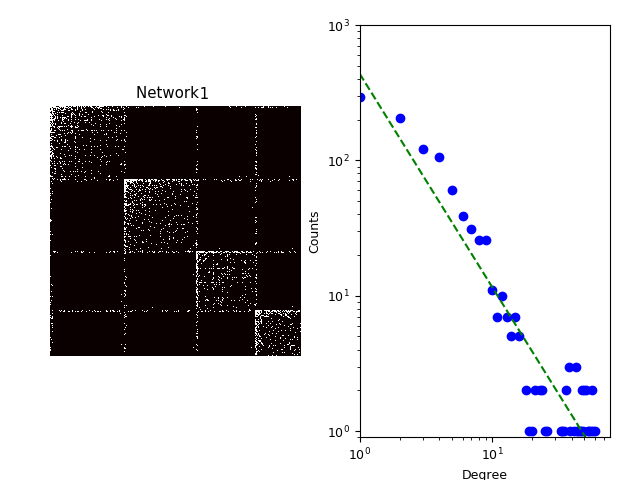
\includegraphics[width=\textwidth]{img/corpus/network1_dd}
        \end{minipage}
        \begin{minipage}{0.24\textwidth}
            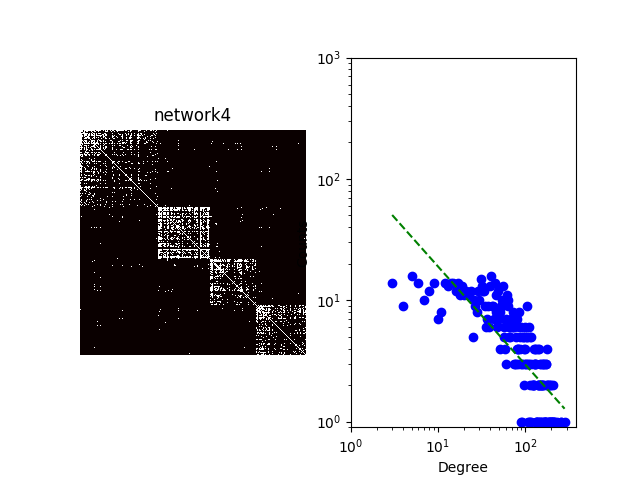
\includegraphics[width=\textwidth]{img/corpus/network4_dd}
        \end{minipage}
        \vskip\baselineskip
        \begin{minipage}{0.24\textwidth}
            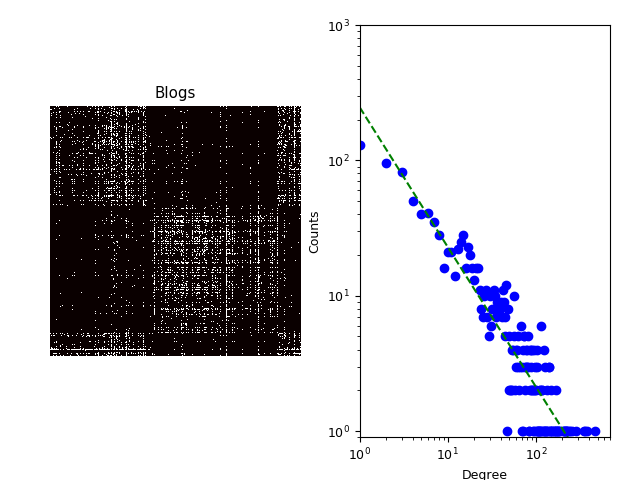
\includegraphics[width=\textwidth]{img/corpus/blogs_dd}
        \end{minipage}
        \begin{minipage}{0.24\textwidth}
            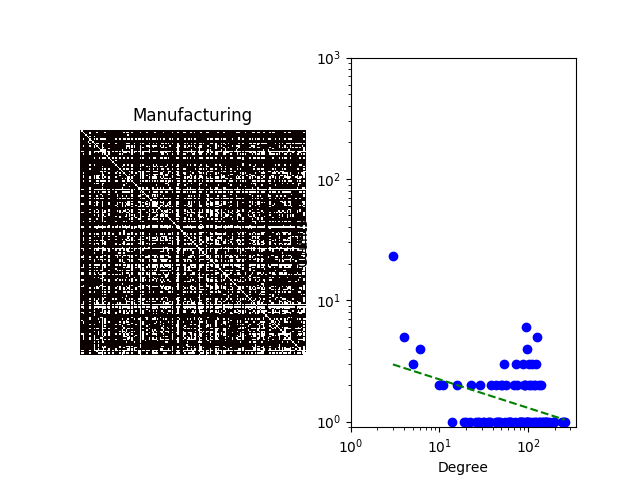
\includegraphics[width=\textwidth]{img/corpus/manufacturing_dd}
        \end{minipage}
	\caption{Adjacency matrices (left) and global degree distributions (right) for the networks datasets.}
	\label{fig:corpuses}
\end{figure}


\begin{figure}[h]
        \begin{minipage}{0.24\textwidth}
            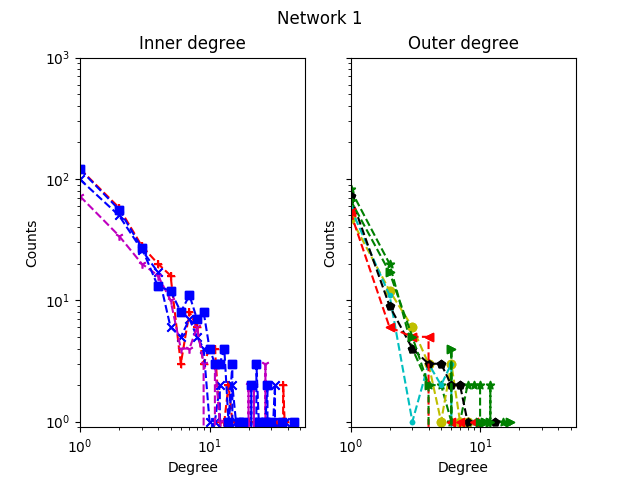
\includegraphics[width=\textwidth]{img/corpus/network1_1}
        \end{minipage}
        \begin{minipage}{0.24\textwidth}
            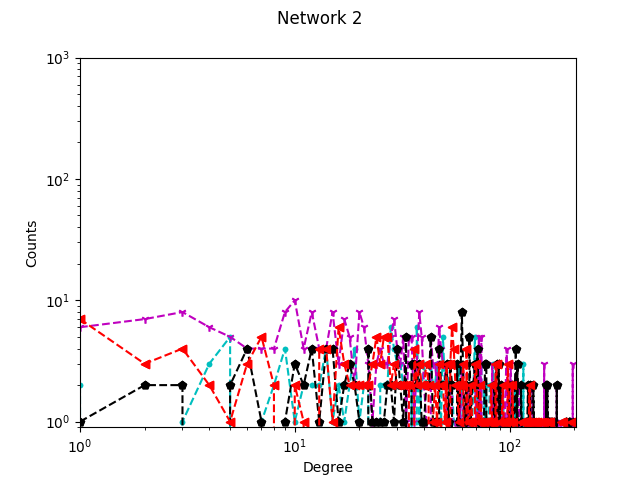
\includegraphics[width=\textwidth]{img/corpus/network2_1}
        \end{minipage}
        \vskip\baselineskip
        \begin{minipage}{0.24\textwidth}
            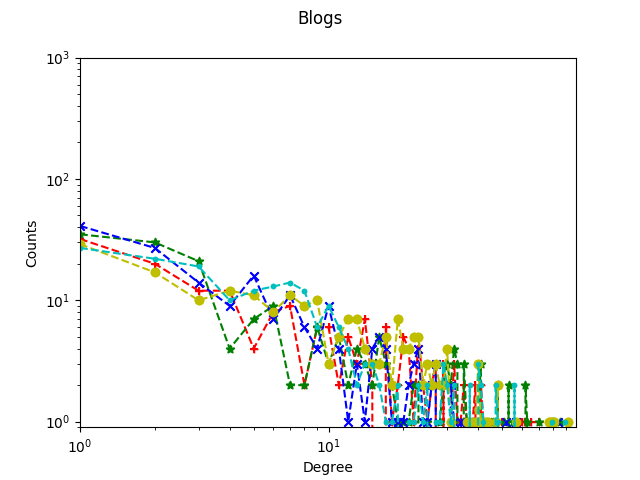
\includegraphics[width=\textwidth]{img/corpus/blogs_1}
        \end{minipage}
        \begin{minipage}{0.24\textwidth}
            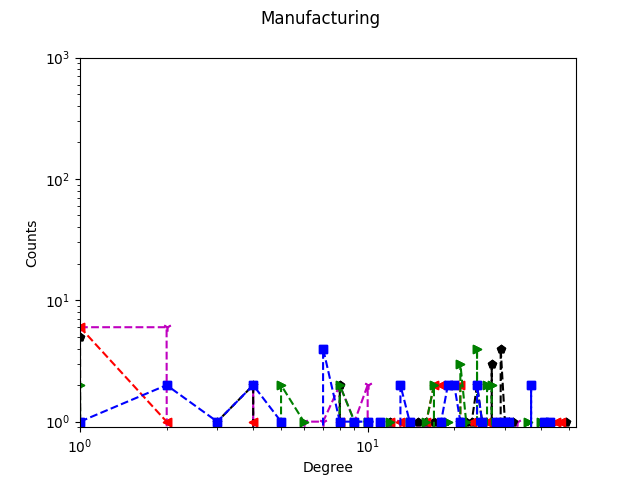
\includegraphics[width=\textwidth]{img/corpus/manufacturing_1}
        \end{minipage}
        \caption {Local degree distributions for the four networks datasets. Inner(left) and outer(right) degree are separated. For Network1 and Network2 the classes come from ground-truth. For Blogs and Manufacturing we use classes find by a Louvain algorithms.} 
	\label{fig:synt_graph_local}
\end{figure}




\subsection{Model Evaluation}
For each dataset described earlier, we run a MCMC inference consisting of 200 iterations to learn the posterior distribution for the IMMSB and ILFM  models described previously. For IMMSB, the concentration parameters of HDP were optimized  using vague gamma priors $\alpha_0 \sim \text{Gamma}(1,1)$ and $\gamma \sim \text{Gamma}(1,1)$ following \cite{HDP}. The parameters for the matrix weights  $\lambda_0$ and $\lambda_1$ were fixed to 0.1. For ILFM, the weights hyperparameter  $\sigma_w$ was fixed to 1 and the IBP hyperparameter $\alpha$ to 0.5 in order to  have comparable number of classes with IMMSB.

The inference procedure was run with these settings for ten runs, and the following experiments are averaged on them.

This inference procedure was run ten times and the average values are reported as final results.

Table \ref{table:me_gofit} reports the value of the power-law goodness of fit for IMMSB and ILFM in the global case (left) and in the local case (right). To compute those statistics we use the model in generative mode over all the nodes. Thus we obtain a fully generated networks from the models parameters $\hat F$ and $\hat \Phi$. Note that the $p$-values statistic for the \emph{local} settings are averaged over all classes.

It appears that for the both models, the global preferential attachment is only verified in the generated networks learned from datasets where the property was verified, namely in Network1 with p-value equals to 0.9 for IMMSB and 1 for ILFM, and in Blogs with a p-value equals to 1 for the both models whereas the property is not verified in Network2 and in Manufacturing (p-value = 0). This is in accordance with Proposition 2.1  according which both ILFM and IMMSB do not satisfy global preferential attachment. However these models are able to capture this property if it exists in the learning dataset.  Moreover we can observed that, in the local case, IMMSB complies with the preferential attachment with a close-to-one $p$-value for the four networks while ILFM obtained low p-values for the networks that were less locally bursty with a value of 0 and 0.3 respectively for Network2 and Manufacturing. Also, the mean value of the power-law coefficient $\alpha$ is significantly greater for IMMSB than for ILFM and specially for the bursty networks, Network1 and Blogs.

The figure \ref{fig:me_local} illustrates the local preferential attachment by plotting the local degree distributions for the artificial networks Network1 (top) and Network2 (bottom) learned with IMMSB (left) and ILFM (right). The shape of local degree distribution appears more linear for IMMSB and with more fluctuations for ILFM. This illustrates the inability  of ILFM to capture local preferential attachment property,  as stated in Proposition 2.2. 
 

\begin{table}[t]
    \caption{Power law goodness of fit results for the preferential attachment for training datasets and networks generated by fitted models.}
\centering
  \begin{tabular}{lrrrr}
      \multirow{2}{*}{\textbf{Training Datasets}}  &
      \multicolumn{2}{c}{Global} & \multicolumn{2}{c}{Local}\\
      \cmidrule(r){2-3} \cmidrule(l){4-5}
      &   $p$-value &   $\alpha$   & $p$-value & $\alpha$   \\
  	\hline
    Network1       & 1 & 2.4 &   1.0 $\pm$ 0.0  &  1.8 $\pm$ 0.03  \\
    Network2       & 0 & 1.3 &   0.0 $\pm$ 0.0  &  1.2 $\pm$ 0.01 \\
    Blogs          & 1 & 1.5 &   1.0 $\pm$ 0.0  &  1.4 $\pm$ 0.03\\
    Manufacturing  & 0 & 1.4 &   0.4 $\pm$ 0.3  &  1.3 $\pm$ 0.05 \\
  	\hline

      \ \textbf{IMMSB} &&&& \\
  	\hline
    Network1       & 0.9 & 1.4 &   1.0 \(\pm\) 0.0   &  3.5 \(\pm\) 0.7 \\
    Network2       & 0 & 1.3 &   0.9 \(\pm\) 0.0   &  1.6 \(\pm\) 0.2 \\
    Blogs          & 1 & 1.3 &   1.0 \(\pm\) 0.0   &  4.3 \(\pm\) 1.1 \\
    Manufacturing  & 0 & 1.2 &   0.9 \(\pm\) 0.01  &  1.6 \(\pm\) 0.1 \\
  	\hline

      \ \textbf{ILFM} &&&& \\
  	\hline
    Network1      & 1 & 1.4 &   1.0 \(\pm\) 0.0  &  1.7 \(\pm\) 0.1 \\
    Network2      & 0 & 1.2 &   0.0 \(\pm\) 0.0 &  1.2 \(\pm\) 0.0 \\
    Blogs         & 1 & 1.3 &   0.9 \(\pm\) 0.2  &  1.5 \(\pm\) 0.1 \\
    Manufacturing & 0 & 1.2 &   0.3 \(\pm\) 0.3  &  1.3 \(\pm\) 0.0 \\
  	\hline
  \end{tabular}
\label{table:me_gofit}
\end{table}

\begin{figure}[h]
        \begin{minipage}{0.24\textwidth}
            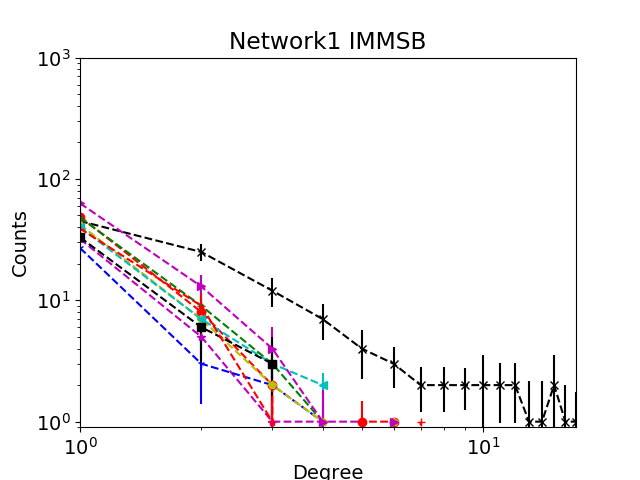
\includegraphics[width=\textwidth]{img/corpus/immsb_network1_1}
        \end{minipage}
        \begin{minipage}{0.24\textwidth}
            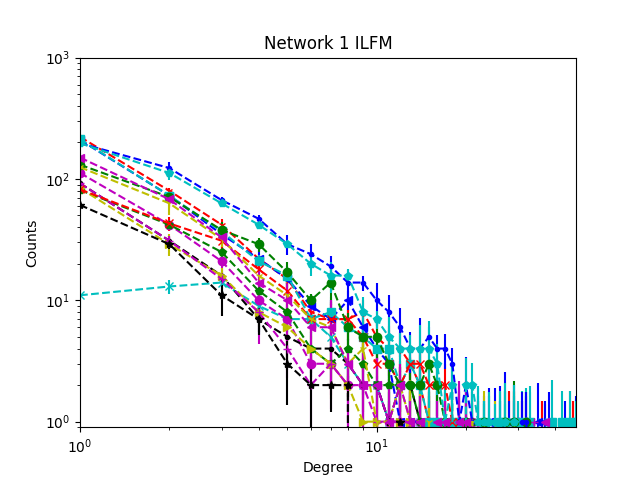
\includegraphics[width=\textwidth]{img/corpus/ilfm_network1_1}
        \end{minipage}
        \vskip\baselineskip
        \begin{minipage}{0.24\textwidth}
            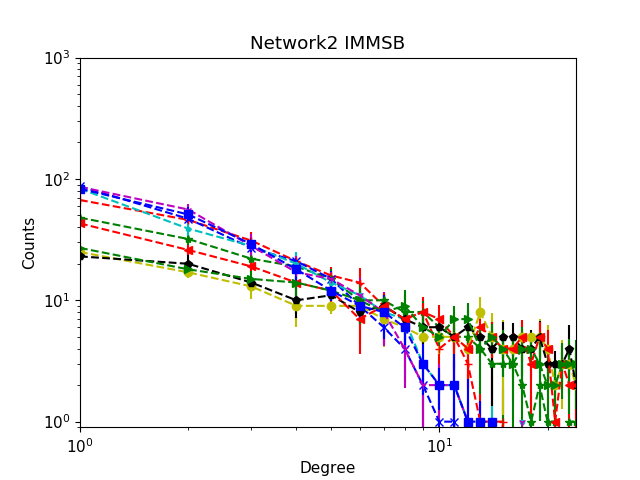
\includegraphics[width=\textwidth]{img/corpus/immsb_network2_1}
        \end{minipage}
        \begin{minipage}{0.24\textwidth}
            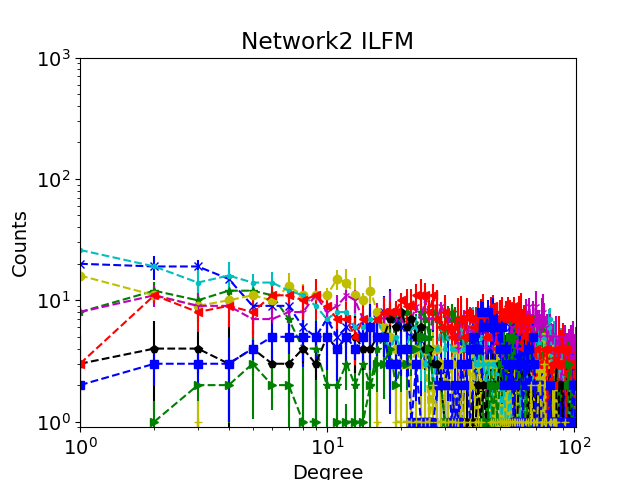
\includegraphics[width=\textwidth]{img/corpus/ilfm_network2_1}
        \end{minipage}
        \caption {Local degree distribution for of fitted models for Network1 (top row) and Network2 (bottom row) learned by IMMSB (first column) and ILFM (second column).} 
	\label{fig:me_local}
\end{figure}

Figure \ref{fig:homo_mustach} presents boxplots describing the distributions of the similarity natural $s_n(i,j)$ and latent $s_l(i,j)$ computed respectively on linked and non-linked pairs of nodes and averaged over 10 networks generation with IMMSB (left) and ILFM (right). The results have been aggregated over the four datasets.  It confirms that the natural similarity is  higher for  pairs of nodes which are connected than between nodes which are not linked for both models. However, we can noticed that for IMMSB, the similarities computed on the non linked pairs are more concentrated around zero which provides an interesting insight of the bursty behavior of this model. For the latent similarity,  there is no difference between the linked and not linked pairs, and consequently, we can not say that similar nodes are more likely to be connected. These experimental results are in accordance with our theoretical results presented in Section \ref{sec:homophily} which state that both ILFM and IMMSB are homophilic with respect to the natural similarity $s_n(i,j)$ and are not homophilic for the latent similarity $s_l(i,j)$ .
\begin{figure}[h]
    \centering
        \begin{minipage}{0.24\textwidth}
            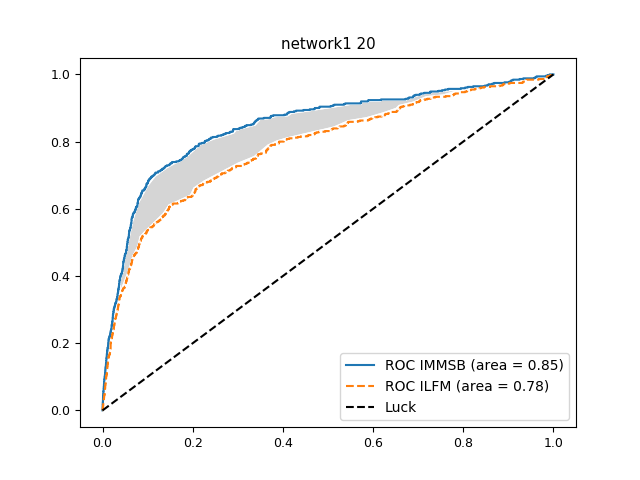
\includegraphics[width=\textwidth]{img/corpus/roc_network1_20_f}
        \end{minipage}
        \begin{minipage}{0.24\textwidth}
            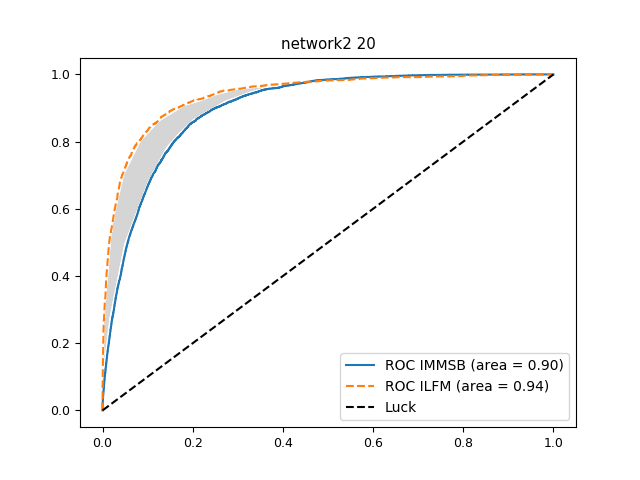
\includegraphics[width=\textwidth]{img/corpus/roc_network2_20_f}
        \end{minipage}
        \begin{minipage}{0.4\textwidth}
            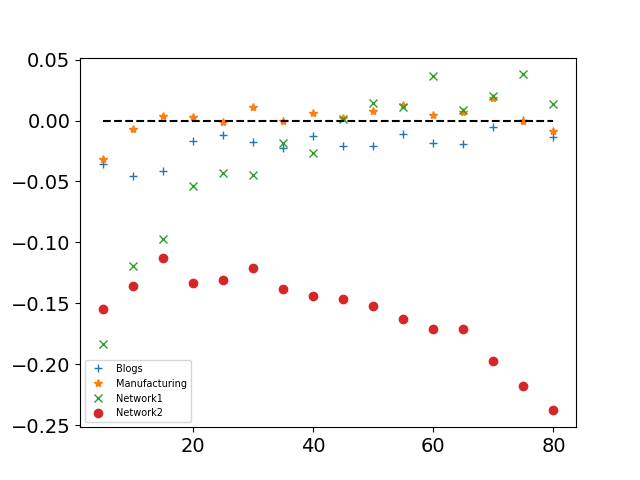
\includegraphics[width=\textwidth]{img/corpus/testset_max_20.png}
        \end{minipage}
        \caption{The two upper top figures represent AUC-ROC curves that compares ILFM and IMMSB on Network1 and Network2. The bottom figure is the relative AUC values when the size of the training set decrease. The y-axis represents the difference of max AUC values obtains for ILFM and IMMSB on ten inference trial. The x-axis label indicates the number precentage of sampled removed from the training set and used for the testing set. } 
	\label{fig:auc}
\end{figure}


Figure \ref{fig:auc} compares the performances of the models on the different datasets in function of  the training set size. Indeed, in the bottom Figure, the y-axis gives the relative performance defined as the difference of the AUC values obtained for IMMSB and ILFM: $AUC_{IMMSB} - AUC_{ILFM}$ whereas the x-axis indicates by the percentage of data (links) randomly removed from the datasets and  used as  testing set. Hence the number of training data decreases with the x-axis and a positive value on the y-axis indicates that IMMSB outperforms ILFM. The two top graphs on figure \ref{fig:auc} illustrate this relative perfomance with a grey zone, where for Network1 (left) IMMSB dominate ILFM and the opposite for Network2 (right). Note that the relative performances over the training set size (bottom graph), represent the difference of the MAX AUC values obtained for both models for the 10 inferences experiences.


This figure shows that for bursty networks, the predictive performance of IMMSB increases when the quantity of training data decreases whereas for non-bursty networks, the results are the opposite: the performance of ILFM increases when the size of the learning data decreases. This is particularly visible for Network2, more contrasted for Manufacturing,  probably due to the small size of this last network which makes the comparison more difficult.



\begin{figure}[h]
    \centering
        \begin{minipage}{0.24\textwidth}
            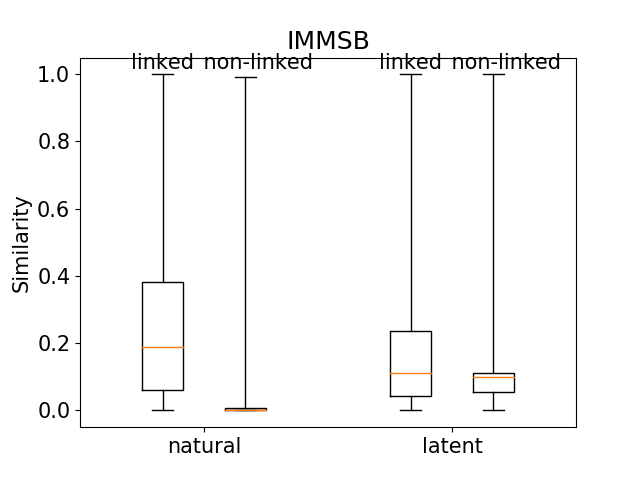
\includegraphics[width=\textwidth]{img/corpus/homo_mustach_immsb}
        \end{minipage}
        \begin{minipage}{0.24\textwidth}
            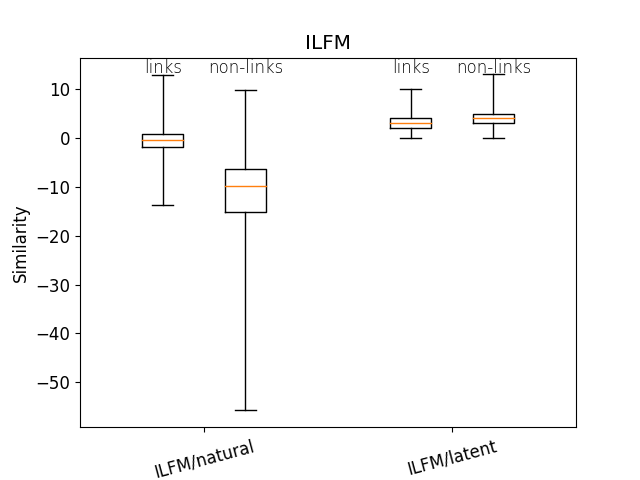
\includegraphics[width=\textwidth]{img/corpus/homo_mustach_ilfm}
        \end{minipage}
        \caption{Boxplot for IMMSB (left) and ILFM (left) of the distributions for natural and latent similarities on the overall datasets separated for links, and non-links observations. }
        \label{fig:homo_mustach}
\end{figure}


